
\chapter{Инфраструктура}
\label{ch:infrastructure}

В данной главе подробно рассмотрены детали масштабируемой архитектуры приложения.

\section{Внутренние сервера}
\subsection{Старт нового сервера}
	При автоматическом запуске машины на Amazon мы можем небольшое количество информации, а именно, идентификатор AMI и User Data - небольшой набор инструкций, который будет выполнен после запуска. Данный параграф посвящён тому, как при помощи этого небольшого количества данных можно настроить компьютер и запустить приложение.
	
	Для того, чтобы просто запустить компьютер, нам достаточно идентификатора AMI. Первоначально нами был выбран образ с CoreOS, т.к. планировалось запускать приложение внутри докер-контейнера, а CoreOS как раз предназначена для таких случаев.
	
	После того, как мы запустили компьютер нам необходимо скачать наше приложение и его окружение.Теоретически, всё приложение вместе с окружением можно было бы поместить внутрь одного докер образа, а при старте машины запустить докер-контейнер, основанный на нём. Проблема такого подхода заключается в том, что при обновлении исходного кода приложения, что происходит очень часто, нам приходилось бы добавлять дополнительный слой, что приводило бы к сильному росту размера образа.
	
	С учётом этого был применён несколько другой подход, при котором вся необходимая инфраструктура и настройки, которые меняются достаточно редко, помещаются в докер образ, а само приложение хранится в Amazon S3Bucket - облачном файловом хранилище Amazon. В такой ситуации при старте машины нам необходимо  скачать наше приложение из S3 при помощи соответствующего приложения, запущенного внутри докер контейнера. После этого мы можем запускать основной контейнер, который основывается на образе с настройками, и передать ему скачанное приложение.
	
	Все необходимые докер-контейнеры запускаются в виде системного сервиса (см. systemd). Это позволяет сохранить информацию об ошибках, возникших при исполнении контейнеров. Также при таком подходе контейнер с приложением может быть автоматически перезапущен в случае если его исполнение завершилось с ошибкой.
	
	В результате получается следующее описание сервиса, являющееся основной частью User Data:
\begin{lstlisting}
[Unit]
Description=Kotlin web Demo backend Green
After=docker.service

[Service]
TimeoutStartSec=1800s
Restart=always
ExecStartPre=-/usr/bin/docker rm -f war-container-green
ExecStartPre=/usr/bin/docker run --name=war-container-green -v /wars docker-registry.labs.intellij.net/itops/aws-cli s3 cp s3://kotlin-web-demo-backend/green/WebDemoBackend.war /wars
ExecStartPre=/usr/bin/docker pull docker-registry.labs.intellij.net/kotlin/web-demo-backend
ExecStart=/usr/bin/docker run -m="1536m" --rm=true -e "LFS_NAME=kotlin.web.demo.backend" --name tomcat-green --volumes-from war-container-green -p 8080:20039 docker-registry.labs.intellij.net/kotlin/web-demo-backend

ExecStop=/usr/bin/docker stop tomcat-green
\end{lstlisting}

\subsection{Выбор типа виртульной машины}
	%TODO: всюду "тип"
	Одним из параметров конфигурации запуска виртуальной машины на Amazon является её тип. Он определяет то, насколько мощный будет CPU, количество памяти и.т.д.. Также от него зависит стоимость~--- чем лучше параметры, тем дороже стоит виртуальная машина, что делает выбор типа  важным этапом создания инфраструктуры на Amazon.
	
	В таблице \ref{table:instance_types} приведены основные характеристики тех типов, которые рассматривались в качестве кандидатов.
	
	Как видно, CPU у ряда типов виртуальных машин, а именно, у машин типа t2, помечены Burstable. Это~--- возможность временно увеличивать производительность CPU, тратя при этом кредиты CPU. Кредиты CPU -- это абстракция, использующаяся Amazon. Они копятся со временем и теряются либо при большом потреблении CPU, либо по истечении суток. Подобная система разработана для приложений, у которых в среднем нагрузка мала, однако периодически она может возрастать.
	
\begin{table}[ht]
	\centering
	\begin{tabular}{l|c|c|c}
		Type      & CPU Units    & Memory & Cost\\ \hline
		t2.small  & 1(Burstable) & 2GB    & \$0.026 hourly\\ \hline
		t2.medium & 2(Burstable) & 4GB    & \$0.052 hourly\\ \hline
		m3.medium & 3            & 3.75GB & \$0.070 hourly\\ \hline
		c4.large  & 8            & 3.75GB & \$0.116 hourly\\
	\end{tabular}
	\caption{Параметры интересующих нас типов амазоновских инстансов}
	\label{table:instance_types}
\end{table}
	
	Для сравнения производительности виртуальных машин использовались два простых нагрузочных теста. В обоих тестах на сервер посылались запросы на исполнение ``Hello, World!'' программы. В первом случае запросы постоянно отправлялись из одного потока, и измерялось время обработки каждого запроса. Во втором случае измерялось максимальное количество потоков, при котором сервер успевал исполнять программу (через 5 секунд после старта программа завершается).
	
\begin{table}[ht]
	\centering
	\begin{tabular}{l|c|c}
		Type      & Время обработки запроса    & Максимальное число потоков\\ \hline
		t2.small  & 0.5(Burst)/2.5             & 7(Burst)/1  \\ \hline
		t2.medium & 0.5(Burst)/2.5             & 15(Burst)/2 \\ \hline
		m3.medium & 1.2                        & 4           \\ \hline
		c4.large  & 0.5                        & 10          \\
	\end{tabular}
	\caption{Параметры интересующих нас типов виртуальных машин Amazon}
	\label{table:instance_types_performance}
\end{table}

	Из двух приведённых выше таблиц видно, что нам явно не подходят m3.medium инстансы, т.к. у них стабильно низкая мощность CPU.
	
	Намного интересней всё с виртуальными машинами типа t2. Из таблицы \ref{table:instance_types_performance}	 видно, что они могут выдавать производительность даже большую, чем более дорогие машины типа c4.large, но есть очевидная проблема, которая заключается в том, что мы можем потратить все CPU кредиты. Данная проблема наиболее существенна при возникновении достаточно долгой большой нагрузки, т.к. общего числа накопленных кредитов может хватить максимум на час работы при максимальном потреблении CPU. В такой ситуации одна машина перестанет справляться, и система автоматического масштабирования должна будет поднять новые, которые тоже будут типа t2. А это означает, что каждая поднятая машина в таких условиях сможет нормально работать только в течение часа, после чего она станет почти бесполезной. 
	
	Также существует ещё одна связанная с кредитами проблема. Ресурсом, который мы активней всего тратим, является CPU, поэтому и наши метрики, которые отвечают за масштабирование, настроены на то, чтобы смотреть на потребление CPU. Когда у машины типа t2 кончаются кредиты, уровень потребления CPU у неё не поднимается выше 20\%. Это приводит к тому, что согласно нашим метрикам, нагрузка на систему мала, а значит и новые машину поднимать не нужно. Данная ситуация является катастрофичной, т.к. сервера не смогут обрабатывать запросы в связи с тем, что они перегружены, а система масштабирования будет считать, что всё нормально и ничего не предпринимать, что приведёт к неработоспособности приложения до тех пор, пока не спадёт нагрузка.
	
	Учитывая всё вышесказанное, можно сказать, что машины типа t2 обладают очень хорошим соотношением мощности к цене, однако в сколь бы то ни было серьёзном приложении их использование представляется невозможным в связи с их ненадёжностью. Учитывая это, а так же тот факт , что тип m3.medium обладает очень слабым процессором, в итоге были выбран тип с4.large.
\subsection{Подбор метрик}
	Как было сказано ранее, автоматическое масштабирование в Amazon основано на событиях Cloud Watch Alarm, каждое из которых говорит о том, что потребление определённого ресурса было больше/меньше определённого уровня.
	
	%TODO: либо "учитывая это, мы сделали ...", либо "с учётом этого было сделано ... "
	Как показал мониторинг нашего приложения, единственным значимым ресурсом является процессорное время. С учётом этого были созданы соответствующие события:
\begin{itemize}
	\item Если среднее потребление CPU больше 80\% в течение 2 минут, то увеличить количество экземпляров в 2 раза, после чего подождать одну минуту перед следующим масштабированием.
	\item Если среднее потребление CPU меньше 40\% в течение часа, то уменьшить количество экземпляров на 1, после чего подождать пять минут перед следующим масштабированием.
\end{itemize}

	При срабатывании первого события система автоматического масштабирования должна увеличить количество машин в 2 раза, после чего в течение минуты не предпринимать никакой активности.
	
	При срабатывании второго события система должна уменьшить количество машин на 1, после чего подождать пять минут перед следующим масштабированием.

	Из предыдущих абзацев видно, что существенно различается время ожидания перед запуском новых машин и перед уничтожением старых. Это позволяет избежать ситуации, при которой мы будем останавливать только что запущенные машины из-за того, что немного уменьшилась нагрузка, а потом запускать их обратно, т.к. нагрузка обратно возросла. Кроме того, при каждом старте новой машины на Amazon оплачивается один час её работы, что делает подобный подход ещё более осмысленным.
	
	Выбранная нами политика масштабирования является очень агрессивной, т.е. она очень мало ждёт перед поднятием новых машин и увеличивает их количество в геометрической прогрессии. Это сделано для того, чтобы мы могли оперативно среагировать на резко увеличившуюся нагрузку. Недостатком такого подхода является возможность запуска большого количества лишних машин при случайном превышении порога, но в случае нашего приложения этот недостаток не проявляется, т.к. средняя нагрузка на наше приложение значительно меньше порога.
	
\subsection{Время запуска машины. Использование AMI}
	Время отклика приложения на рост нагрузки зависит не только от того, как мы настроили события в Cloud Watch, но и от того, как долго будет запускаться новая виртуальная машина и сколько времени будет настраиваться наше окружение. 
	
	Время запуска новой машины более-менее постоянно и равно 1-2 минутам, а вот время настройки окружения может быть уменьшено. В первоначальной версии это время составляло порядка 7 минут, что приводило к тому, что суммарное время отклика на рост нагрузки было больше 10 минут (2 минуты для срабатывания события, 2 минуты чтобы запустить машину, 7 минут чтобы настроить инфраструктуру). Основная часть этого времени тратилась на скачивание образов докера, среди которых есть очень объёмный образ операционной системы.
	
	Единственный способ избежать скачивания докер-образов~--- это иметь эти докер образы локально. Это можно сделать, если создать образ работающей машины и использовать его для запуска новых машин. При таком подходе время настройки инфраструктуры удалось сократить до нескольких минут, что привело к суммарному времени около 5 минут. 
\section{Инфраструктура с учётом обновлений}
\subsection{Green Blue deployment}
	Среди многочисленных подходов к обновлению приложения, нами был выбран ``Blue Green Deployment'', при котором существует две версии приложения: активная и пассивная. Схема данного подхода в случае нашего приложения приведена на рис.\ref{fig:green_blue_deployment}.
\begin{figure}[ht]
    \centering
    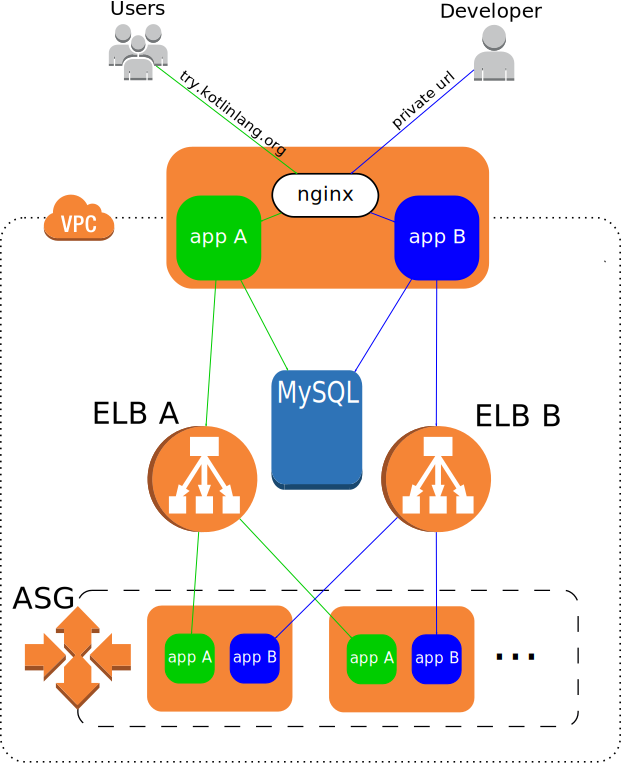
\includegraphics[scale=0.8]{green_blue_deployment} 
    \caption{Детальная схема устройства нашего приложения. Зелёным отмечено активное приложение, синим~--- пассивное}
    \label{fig:green_blue_deployment}
\end{figure}

	Какое приложение является на данный момент активным, определяется в нашей схеме настройками nginx сервера, который принимает все запросы извне. Если запрос был отправлен на публичный адрес try.kotlinlang.org, то он будет перенаправлен активному приложению, а если он был отправлен на адрес, который известен только разработчикам, то он будет перенаправлен в пассивную ветку приложения.
	
	При публикации приложения оно сперва выкладывается в пассивную ветку, после чего проверяется его работоспособность. Если приложение работоспособно, то далее меняются настройки nginx-сервера  и обновлённое приложение становится активным, что завершает процесс публикации обновлений.
\subsection{Выбор стоимость-надёжность}
\label{subsec:deployment_choice}
	Как видно из рисунка \ref{fig:green_blue_deployment}, мы не дублируем никакие машины кроме ELB, которые необходимо дублировать, т.к. они умеют слушать только один порт и отправлять запросы тоже только на один порт. Такая схема является экономичной, однако имеет свои недостатки.
	
	Основным минусом такой схемы является то, что при возникновении проблем в пассивной версии приложения могут возникнуть проблемы в активной версии, связанные с тем, что оба приложения работают внутри одной и той же виртуальной машины.
	
	На внешнем сервере подобной проблемы нет, т.к. каждое из приложений работает внутри своего докер-контейнера, и если в одном из них происходит ошибка, то второе ничего не замечает, т.к. они работают в изолированном окружении.
	
	На внутренних серверах всё было бы точно так же, если бы внутренние сервера не проверялись постоянно на работоспособность балансировщиком нагрузки. Это приводит к тому, что если одно из наших приложений не отвечает по какой-то причине (зависание в процессе публикации, выложена плохое приложение и т.д.), то данный компьютер будет остановлен, а на смену ему будет поднят новый. В худшем случае с новым компьютером всё может повториться и система автоматического масштабирования так и будет запускать и останавливать новые компьютеры, пока мы не починим приложение.
	
	Самым простым решением данной проблемы является копирование инфраструктуры для пассивного приложения, но в такой ситуации нужно тратить дополнительные деньги на работу экземпляров пассивной ветки.